\section{Skew Void-to-Absorber Test Problem}

In this section, results are presented for the skew void-to-absorber test
problem described in Section \ref{sec:skew_void_to_absorber}, where
``skew'' refers to the transport direction, which is no longer
along the $+x$ direction, as in the non-skew void-to-absorber problem
described in Section \ref{sec:void_to_absorber}.
Table \ref{tab:skew_void_to_absorber_run_parameters} shows the run parameters used
to obtain these results, and Figure \ref{fig:skew_void_to_absorber_2D}
shows 2-D and results for this problem.

This test problem reveals some multidimensional effects of spurious
oscillations, as one can see in the Galerkin and EV solutions. Comparing
Figures \ref{fig:skew_void_to_absorber_2D} and \ref{fig:void_to_absorber_2D},
one can see that in the skew case, oscillations are now not just perpindicular
to the $x$ axis but also to the $y$ axis, due to the gradients on each
edge of the absorber region. One can also see some faint oscillations
propagating from the corner of the absorber region. It is also interesting
to note a circular effect centered at the lower left corner of the domain;
this is presumed to be due to interactions between the horizontal and
vertical oscillations. Also note that in this problem, the wave front
is not at the right edge of the domain as it was in non-skew test
problem; instead, the wave front is in the absorber region, which
one can clearly see in the exact solution. The wave front is an ``L''
shape since with the skew, particles/photons now also enter the domain
from the lower boundary of the domain. The conclusion of the results
is the same as before: FCT eliminates the spurious oscillations apparent
in the Galerkin and EV solutions and is sharper than the low-order
solution. The advantage of using FCT over the low-order scheme is
less evident in these results simply because the wave front is
in the absorber region, where the solution is already very small;
thus the gradient is more difficult to see. Also, note that the same
color scheme was used in
Figures \ref{fig:skew_void_to_absorber_2D} and \ref{fig:void_to_absorber_2D};
the range of values is just larger for the non-skew problem due to the
severe oscillations along the lower edge of the absorber region.
%-------------------------------------------------------------------------------
\begin{table}[h]\caption{Skew Void-to-Absorber Test Problem Run Parameters}
\label{tab:skew_void_to_absorber_run_parameters}
\centering
\begin{tabular}{l l}\toprule
\emph{Parameter} & \emph{Value}\\\midrule
Number of Cells & $N_{cell} = 2^5 \times 2^5 = 1024$\\
End Time & $t = 1$\\
CFL Number & $\nu = 0.5$\\
Time Integrator & SSPRK33\\\midrule
Entropy Function & $E(u) = \frac{1}{2}u^2$\\
Entropy Residual Coefficient & $c_E = 0.1$\\
Entropy Jump Coefficient & $c_J = 0.1$\\
Entropy Time Integrator & BE\\
\bottomrule\end{tabular}
\end{table}
%-------------------------------------------------------------------------------
\begin{figure}[h]
   \centering
   \begin{subfigure}{0.3\textwidth}
      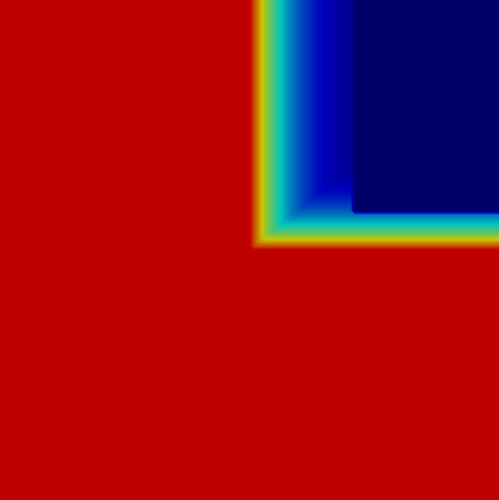
\includegraphics[width=\textwidth]{skew_void_to_absorber/exact.png}
      \caption{Exact}
   \end{subfigure}
   \begin{subfigure}{0.3\textwidth}
      
\includegraphics[width=\textwidth]{skew_void_to_absorber/Gal.png}
      \caption{Galerkin}
   \end{subfigure}
   \begin{subfigure}{0.3\textwidth}
      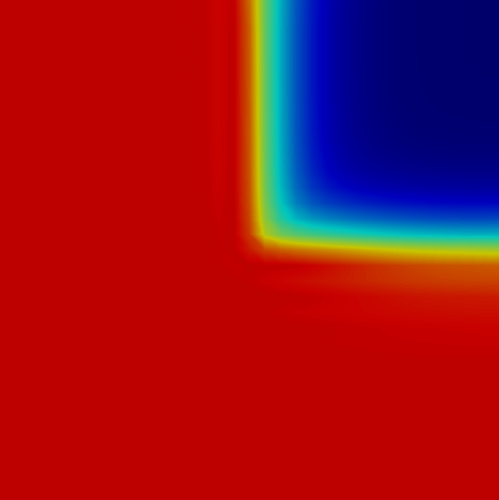
\includegraphics[width=\textwidth]{skew_void_to_absorber/GalFCT.png}
      \caption{Galerkin with FCT}
   \end{subfigure}
   \begin{subfigure}{0.3\textwidth}
      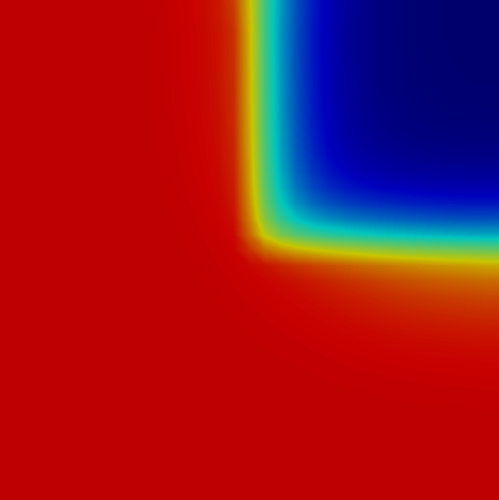
\includegraphics[width=\textwidth]{skew_void_to_absorber/low.png}
      \caption{Low-order}
   \end{subfigure}
   \begin{subfigure}{0.3\textwidth}
      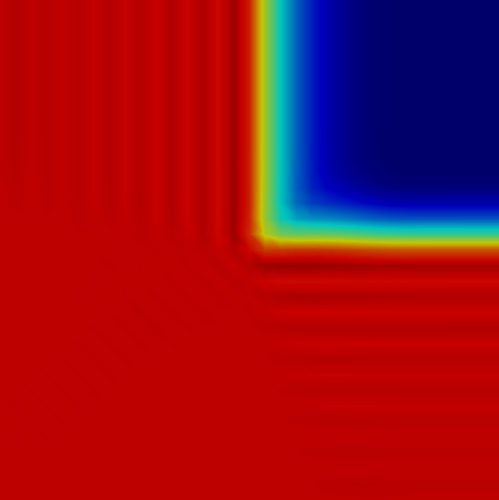
\includegraphics[width=\textwidth]{skew_void_to_absorber/EV.png}
      \caption{Entropy Viscosity}
   \end{subfigure}
   \begin{subfigure}{0.3\textwidth}
      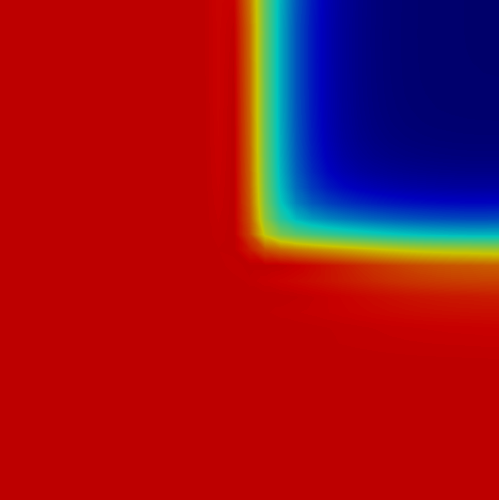
\includegraphics[width=\textwidth]{skew_void_to_absorber/EVFCT.png}
      \caption{Entropy Viscosity with FCT}
   \end{subfigure}
   \caption{Comparison of Solutions for Skew Void-to-Absorber Test Problem}
   \label{fig:skew_void_to_absorber_2D}
\end{figure}
%-------------------------------------------------------------------------------
\subsection{Code and Version}
Deal.ii code, git commit hash bfa12b431d7fdad43ee166a30f3bd56562fc1fa0
